%Latex document for ESSDERC 2021 Paper 

\documentclass[10pt,a4paper,twocolumn]{article}
\usepackage[utf8]{inputenc}
\usepackage{authblk}
\usepackage{amsmath}
\usepackage{nccmath} % added this
\usepackage{amsfonts}
\usepackage{amssymb}
\usepackage{makeidx}
\usepackage{graphicx}
\usepackage[outdir=./]{epstopdf}
\usepackage{fourier}
\usepackage[ruled,vlined]{algorithm2e}
\usepackage{empheq}

\setlength{\parindent}{0pt}
\usepackage[left=1cm,right=1cm,top=1cm,bottom=1.5cm]{geometry}

% Title
\title{PDE and Jitter modelling of SPAD Devices.}

% AUthors and affiliation
\author[1]{Rémi Helleboid}
\author[1]{Denis Rideau}
\author[2]{Isobel Nicholson}
\author[3]{Norbert Moussy}
\author[3]{Olivier Saxod}
\author[1]{Jeremy Grebot}
\author[1]{Antonin Zimmerman}
\author[2]{Sara Pellegrini}	
\author[1]{Matthieu Sicre}

\affil[1]{ST Microelectronics, Crolles, France}
\affil[2]{ST Microelectronics, Edinburgh, UK}
\affil[3]{CEA LETI, Grenoble, France}

\date{}                     %% To hide the date
\setcounter{Maxaffil}{0}
\renewcommand\Affilfont{\itshape\small}
% Keywords command
\providecommand{\keywords}[1]
{
  \small	
  \textbf{\textit{Keywords---}} #1
}


\begin{document}



% Title
\maketitle

% Abstract
\begin{abstract}
In this paper we present a full 3D simulation methodology to extract Photon Detection Probability (PDP) and Jitter of Single-Photon Avalanche Diode (SPAD) Devices. The simulation results are compared with measurements on devices and show good agreement with the experiments.\\
\end{abstract}

% Keywords
\keywords{single-photon avalanche diode (SPAD), photon detection probability (PDP), jitter, avalanche breakdown probability, breakdown voltage}

% Introduction
\section{Introduction}
Single Photon Avalanche Diodes (SPAD) are key optoelectronic detectors for medical imaging, camera ranging and automotive laser imaging detection and ranging (LiDAR) applications. Currently, the device leading the market is a micrometric silicon (Si) PN junction associated to a proximity CMOS electronics biasing the system above the breakdown voltage. Si-SPADs present low noise and relatively high photon detection probability (PDP), but their sensitivity is limited to photon wavelengths lower than 1100 nm, while class 1 eye-safety devices would require wavelengths larger than 1400 nm.


\section{Device structure and TCAD simulation}\label{Device}

A variety of SPAD architectures were devised with pitch size ranging from five to ten microns. Each layout was devised to create a different electric field profile which can vary both laterally and vertically through the full volume of the device. These architectures were manufactured on silicon and characterized using a methodology which prevents contamination of results from any potential crosstalk. 

The structures' doping profiles were modelled with a well-calibrated process simulator followed by electrostatic device simulation. The resulting electric field profiles (calculated as usual by the solution of the Poisson equation) were used as the starting point for a suite of in-house softwares developed to calcuate breakdown probability and jitter characteristics. The carrier density $\rho$ and the recombination-generation processes were computed by resolving current continuity equations consistently with the drift-diffusion transport model. 

In parallel, optical simulation with a well-known FDTD solver was performed on the architectures to obtain maps of optical absorption. The back end of the devices including the microlens and texturation was kept constant for each comparison.

%The modelled devices split into two families. One family was designed with a constant pitch 

%The device structure and its doping profile were implemented in Sentaurus Process . 
%The electric field (F) within the SPAD is calculated by solving the Poisson equation. 

%As indicated on Fig. , the spatial discretization and TCAD outputs were extracted from Sentaurus Device  allowing to interpolate physical fields at each vertex.

%Silicon based SPAD with n-on-p structure is considered as depicted on Fig.1.a. The architecture is composed of n- and p-wells as multiplication region and n- and p-guard rings which prevent premature peripherical breakdown. Passivation at interfaces constrains surface states. Deep-trench isolation (DTI) ensures isolation with environment. A high-k insulator on top limits corrosion, lowers surface dangling bonds and its optical properties ensure optimal photons absorption. 


\section{Avalanche breakdown probability}
The avalanche breakdown probability is computed by the means of the well known McIntyre model \cite{oldham_triggering_1972}. We briefly recall the model derivation : 
Let $P_e(x)$ be the probability that an electron starting at x in the depletion layer triggers an avalanche and $P_h(x)$ the same probability for an hole starting at x.
Straightforwardly, the probability that neither an hole nor an electron starting at x trigger an avalanche is given by $(1-P_e(x))(1-P_h(x))$.
Thus, the probability that either the hole or the electron trigger an avalanche, noted $P_{pair}$ is :
\begin{align*}
P_{pair}(x) &= 1 - \left( 1-P_e(x)\right)\left(1-P_h(x)\right)  \\
			&= P_e + P_h - P_e P_h
\end{align*}

Now, the probability that an electron starting at $x+dx$ triggers an avalanche is :
The probability that the electron reaches the position $x$ and triggers an avalanche in $x$ plus the probability that it triggers an avalanche between $x$ and $x+dx$ less the probability of the intersection of the two previous events. It writes : 
\begin{align*}
P_e(x+dx) &= P_e(x) + \alpha_e(x) dx P_{pair}(x)  - P_e(x)  \alpha_e dx P_{pair}(x) \\
		  &= P_e(x) + \alpha_e(x) dx (P_e(x) + P_h(x) - P_e(x) P_h(x)) \\& \qquad - P_e(x) \alpha_e(x) dx (P_e(x) + P_h(x) - P_e(x) P_h(x)) \\
		  &=  P_e(x) + dx \, \alpha_e(x) (P_e(x) + P_h(x) - P_e(x) P_h(x)) (1 - P_e(x))
\end{align*}
Where $\alpha_e$ is the electron linear ionization rate : the probability by length that an electron create an impact ionization event.  \\
One can rearrange the terms to obtain : 
\[ \frac{P_e(x+dx)-P_e(x)}{dx} = \alpha_e(x) (P_e(x) + P_h(x) - P_e(x) P_h(x)) (1 - P_e(x)) \]
Which leads to the first ordinary differential equation : 
\[ \frac{dP_e}{dx} = (1-P_e)\alpha_e(P_e + P_h - P_e  P_h) \]

The same reasoning applies to the probability that an hole starting at $x-dx$ triggers an avalanche.
Which leads to the second ordinary differential equation : 
\[ \frac{dP_h}{dx} = -(1-P_h)\alpha_h(P_e + P_h - P_e  P_h) \]

Therefore we can draw up the McIntyre system : 

\begin{empheq}[left=\empheqlbrace]{align}
&\frac{dP_e}{dx} = (1-P_e)\alpha_e(P_e + P_h - P_e  P_h) \\
&\frac{dP_h}{dx} = -(1-P_h)\alpha_h(P_e + P_h - P_e  P_h) 
\end{empheq}
for $ 0 \leq x \leq W$. \\
Adding the couple of boundary value conditions
 : 
\begin{empheq}[left=\empheqlbrace]{align}
& P_e(x=0) = 0 \\
& P_h(x=W) = 0 
\end{empheq}
we have a full 1D coupled and non-linear boundary value problem.
Since we have to extract this value at a large number of points, we use a self-made solver, embedded in a C++ program. This solver uses finite difference method coupled with a Newton's method to care of the non-linearity of the problem \cite{ascher_numerical_1987}. 

\subsection{Newton's method}
We set the following notations : 
 \[ Y(x) = \begin{pmatrix}
P_e(x) \\
P_h(x)
\end{pmatrix}
 \]

 \[ f(Y, x) = \begin{pmatrix}
(1-Y_1(x))\alpha_e(Y_1(x) + Y_2(x) - Y_1(x)  Y_2(x)) \\
-(1-Y_2(x))\alpha_h(Y_1(x) + Y_2(x) - Y_1(x)  Y_2(x)) 
\end{pmatrix}
\]

\[ g(s_1, s_2) = \begin{pmatrix}
s_1 \\
s_2
\end{pmatrix} \]

The problem hence reads : 
\begin{empheq}[left=\empheqlbrace]{align}\label{BVP_Prob}
	&Y'(x) = f(Y, x) \\
	&g(Y(0), Y(w)) = 0
\end{empheq}


The numerical method relies on a finite difference method approach to discretize the problem. Let $\mathcal{M}$ be the mesh on which we work. It is given by the streamlines construction. So we have : 
\[\mathcal{M}: 0 = x_1 < x_2 < x_3 < \cdots < x_N < x_{N+1} = w \]
The approximated solution on mesh $\mathcal{M}$ is $Y_{\mathcal{M}} = (y_1, y_2, \cdots, y_N, y_{N+1})$, where $y_i$ is the approximation of $Y(x_i)$.\\
For numerical approximation we again consider the mesh $\mathcal{M}$ and denote the vector of approximate solution values at mesh points by $Y_{\mathcal{M}}$. The trapezoidal scheme of finite difference methods is given by : 
\begin{align}\label{TrapezScheme}
&\frac{y_{i+1}-y_{i}}{h_{i}}=\frac{1}{2}\left(f\left(x_{i+1}, y_{i+1}\right)+f\left(x_{i}, y_{i}\right)\right) \quad 1 \leq i \leq N \\
&\quad g\left(y_{1}, y_{N+1}\right)=0
\end{align}
Thus we obtain a system of $2(N +1)$ algebraic equations for the $2(N +1)$ unknowns $Y_{\mathcal{M}}$. Unlike before, though, these equations are non-linear. The number $N$ depends on the precision we take when we construct the streamlines. We commonly take a range of $\left[1nm, 10nm\right]$, we then have $N \sim 5000$. \\
We consider a system of equation written in the compact form : \[ \textbf{F(s) = 0} \]
%We define a function \textbf{G} : 
%\[  \textbf{G}(\textbf{s}) = \textbf{s^k} - \left[\textbf{F}'(\textbf{s^k}) \right]^{-1} \textbf{F}(\textbf{s^k})\]
%with $\textbf{F}'(\textbf{s})^{-1} $ the inverse of the Jacobian matrix of F : 
%\[\textbf{F}'(\textbf{s}) = \frac{\partial\textbf{F}(\textbf{s}) }{\partial \textbf{s}}  \]

Then the newton method iterative method is given by the  iteration : 
\[\textbf{s}^{k+1} =  \textbf{s} - \left[\textbf{F}'(\textbf{s}) \right]^{-1} \textbf{F}(\textbf{s}) \]
with $\textbf{F}'(\textbf{s})^{-1} $ the inverse of the Jacobian matrix of $\textbf{F}$. \\ 
So the algorithm will first solve the linear system : 
\begin{equation}
\mathbf{F}^{\prime}\left(\mathbf{s}^{k}\right) \boldsymbol{\xi}=-\mathbf{F}\left(\mathbf{s}^{k}\right)
\end{equation} 
And then simply applies : 
\begin{equation}
\textbf{s}^{k+1} = \textbf{s}^{k} + \boldsymbol{\xi}
\end{equation} 

Let $\textbf{N}_{\mathcal{M}}$ be the following discrete differential operator : 
\[ \textbf{N}_{\mathcal{M}} \textbf{y}_i = \frac{y_{i+1}-y_{i}}{h_{i}}-\frac{1}{2}\left(f\left(x_{i+1}, y_{i+1}\right)+f\left(x_{i}, y_{i}\right)\right) \]

Then \[ \textbf{F}(\textbf{s}) = \begin{pmatrix}
N_{\mathcal{M}}\textbf{y}_1,
N_{\mathcal{M}}\textbf{y}_1,
\dots, 
N_{\mathcal{M}}\textbf{y}_N,
g(y_1, y_{N+1})
\end{pmatrix}
 \] 
We set
\[  \boldsymbol{\xi} = \begin{pmatrix}
\textbf{w}_1 ,
\textbf{w}_2 ,
\dots ,
\textbf{w}_N ,
\textbf{w}_{N+1}
\end{pmatrix}
\]
So that the Newton method iteration becomes : 
\begin{equation}
\frac{\mathbf{w}_{i+1}-\mathbf{w}_{i}}{h_{i}}-\frac{1}{2}\left[A\left(x_{i+1}\right) \mathbf{w}_{i+1}+A\left(x_{i}\right) \mathbf{w}_{i}\right]=-\mathbf{N}_{\mathcal{M}} \mathbf{y}_{i}^{k	} \quad 1 \leq i \leq N
\end{equation}
\begin{equation}
B_{a} w_{1}+B_{b} w_{N+1}=-g\left(y_{1}^{m}, y_{N+1}^{m}\right)
\end{equation}
Where $A$ is the following matrix : 
$$
A\left(x_{j}\right):=\frac{\partial f}{\partial y}\left(x_{j},{\mathbf{y}}_{j}^{k}\right)
$$
And with $$
B_{a}=\frac{\partial g(\mathbf{y_1^k}, \mathbf{y_{N+1}^k})}{\partial \mathbf{u}} = 1, \quad B_{b}=\frac{\partial \mathbf{g}(\mathbf{y_1^k}, \mathbf{y_{N+1}^k})}{\partial \mathbf{v}} = 1
$$

\begin{figure}[hbtp]
\centering
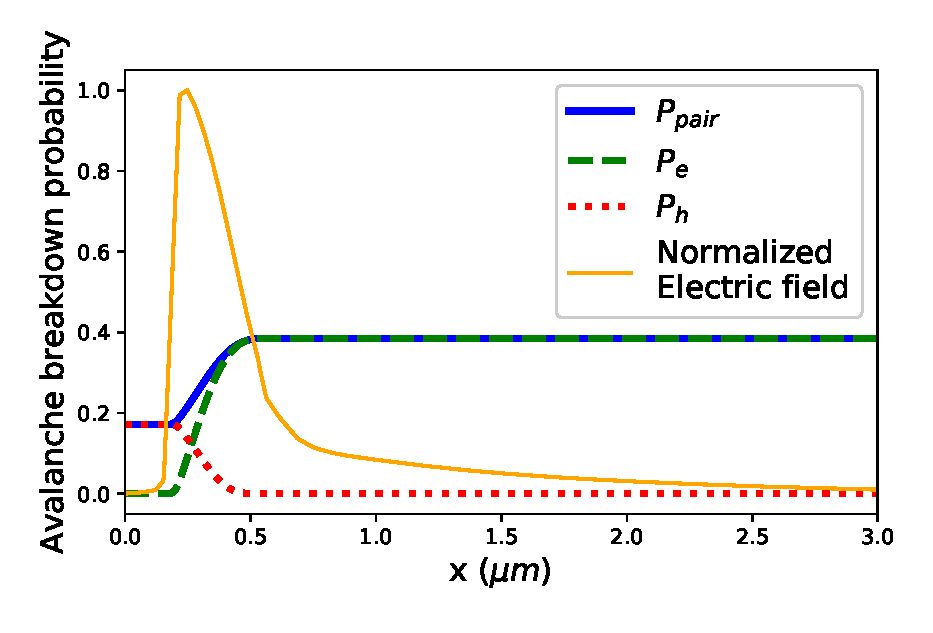
\includegraphics[scale=0.65]{../pictures/PlotStreamline_1_.eps}
\caption{Typical solution of the McIntyre model for a given electric field curve}
\label{fig:BrPOnLine}
\end{figure}


\subsection{Application to field lines}
The McIntyre model is a fully 1D model where the electron and holes path are assumed to be a straight line, often took from the bottom to the top of the device, see for example \cite{panglosse_dark_2020}. In this work we wish to have accurate values of breakdown probability in all the device volume. To this purpose we use electric field streamline to model the carriers transport inside the device. 
%While this modelization might be less accurate than a drift-diffusion model, it would not be consistent with the McIntyre model, where electrons and holes are assumed to follow the same path.
The field lines are computed straightforwardly using simple Euler scheme with adaptive step to ensure a good distribution of points along the line.
\begin{equation}
	\frac{dX(s)}{ds} = \vec{F}_{electric}
\end{equation}
Then the streamline is defined by the following set of points : \[ \{X(s) \text{ for } s \in [s_0, s_f]   \} \]
Our Euler method then reads : 
\begin{align}
	&\frac{X(s+ds)-X(s)}{ds} = \vec{F}_{electric}(X(s)) \\
	\implies & X(s+ds) = X(s) + \underbrace{ds\vec{F}_{electric}(X(s))}_{dX}
\end{align}
%So with the discretization, calling $X^k$ the approximation of $X(k*ds)$ we have : 
%\begin{align}
%&\frac{X^{k+1}-X^k}{ds} = \vec{F}_{electric}(X^k) \\
%\implies & X^{k+1} = X^k + \underbrace{ds\vec{F}_{electric}(X^k)}_{dX^k}
%\end{align}
This operation is performed both forward (hole motion) and backward (electron motion). We then interpolate the electric field on the resulting streamline.
%We set one extremity of the line as it's beginning and the other end as it's end.
We can now obtain a function E(x) where x is the distance from the beginning of the line and E(x) is the norm of the electric field at this point. The streamlines and this function are respectively represented on figures \ref{fig:Streamlines} and \ref{fig:BrPOnLine}




We can now compute the impact ionization coefficients, required to compute the McIntyre's model, in this work we choose the local coefficient from Van Overstraeten and De Man \cite{van_overstraeten_measurement_1970}.

We can compute the breakdown probability over multiple streamlines starting from multiple points inside the device and plot them to have an idea of the breakdown probability inside the device, see figure.

\begin{figure}[h!]
\centering
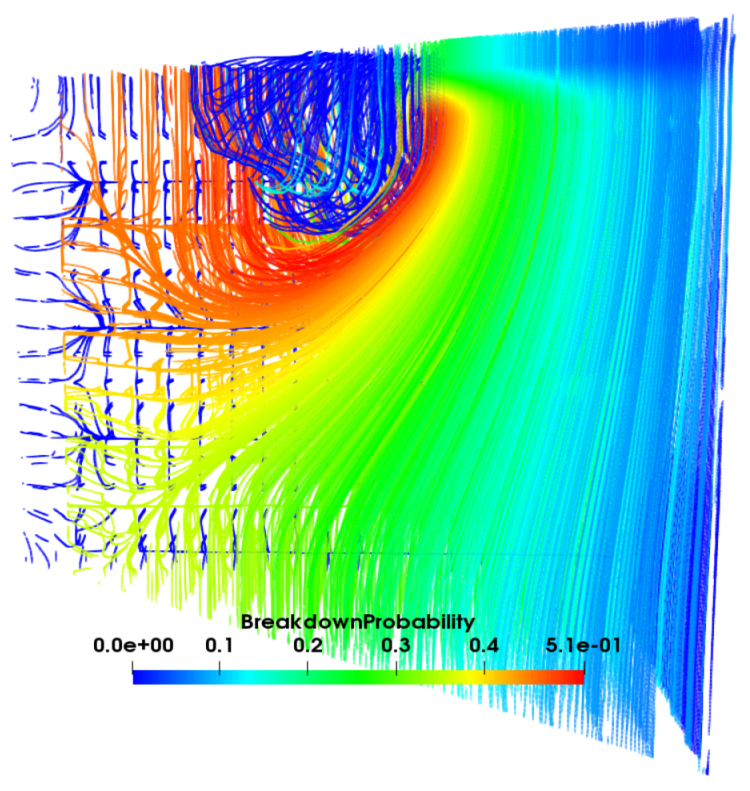
\includegraphics[scale=0.5]{../pictures/BrPStreamlines.PNG}
\caption{Breakdown Probability computed over multiple streamlines}
\label{fig:Streamlines}
\end{figure}





\section{Jitter modeling}
\subsection{Drif-Diffusion model}
The jitter in SPAD devices is made of multiple phenomena such as depth of photon absorption, carrier transport timing, avalanche build-up,quench circuit statistics etc. \\In the present work, we focus on the modeling of the carrier transport part which is responsible for the queue of the jitter  distribution. To do so, we couple the streamlines and the one dimensional advection-diffusion equation with variable velocity and diffusion.
Let us consider that a photon absorption at a given point $x_0$ leads to the creation of an electron-hole pair, we want to simulate the timing for the electron to reach the avalanche zone, we assume that this zone is represented by the location of the maximum electric field, denoted $x_{E_{max}}$ . Let $f : (x,t) \mapsto f(x,t)$ the probability distribution of an electron presence. We assume that the electron will drift and diffuse along the electric field streamline. At time $t=0$, f is a Dirac distribution, in order to be able to compute a solution numerically, we start a time $t_0 = \delta t$ where $\delta t$ is as small as possible. We then take the assumption that $D(x) = D(x_0)$ and $u(x) = u_(x_0)$, and that the analytical solution applies for a very small time interval $\delta t$.

 Hence, f verify the following equation : 
 \[ \forall x \in \left[ x_s, x_{max} \right]  \text{ and } t \in \left[ t_0, T \right] \]
\begin{equation}\label{eq:GeneralAD}
\frac{\partial f}{\partial t}(x,t) = 
	- \frac{\partial( u \cdot f )}{\partial x}(x,t)
	+ \frac{\partial}{\partial x}\left(D \cdot \frac{\partial f }{\partial x}\right)(x,t)
\end{equation}
With the following initial condition : 
\begin{equation}
f(x, t=t_0) = \frac{1}{\sqrt{4 \pi D(x_0) t_0}} exp(-\frac{(x-v(x_0)t_0)^2}{4D(x_0)t_0}
\end{equation}
And setting an absorbing boundary condition at $x_s=x_{E_{max}}$:
\begin{equation}
\frac{\partial f}{\partial t}(x_s,t) = 
	\frac{\partial}{\partial x}\left(D \cdot \frac{\partial( f )}{\partial x}\right)(x_s,t)
\end{equation}
The velocity is computed throw a high field saturation model and the diffusion throw the Einstein relation $D = \frac{\mu k_B T}{q}$, these quantities are represented in figure \ref{fig:VelocityDiffusion}. 
Let $T_e$ the time for the electron to reach the avalanche region. It is straightforward that the probability that $T$ is less than $t$ is:
 \[P_r(t<T) =  F_{Pr}(t) = 1 - \int_{x_0}^{x_{max}} f(x, t) dx \]
From this cumulative distribution function, we can find back the distribution of T:
\begin{equation}
f_T (t) = \frac{F_{Pr}(t)}{dt}
\end{equation}

\begin{figure}[hbtp]
\centering
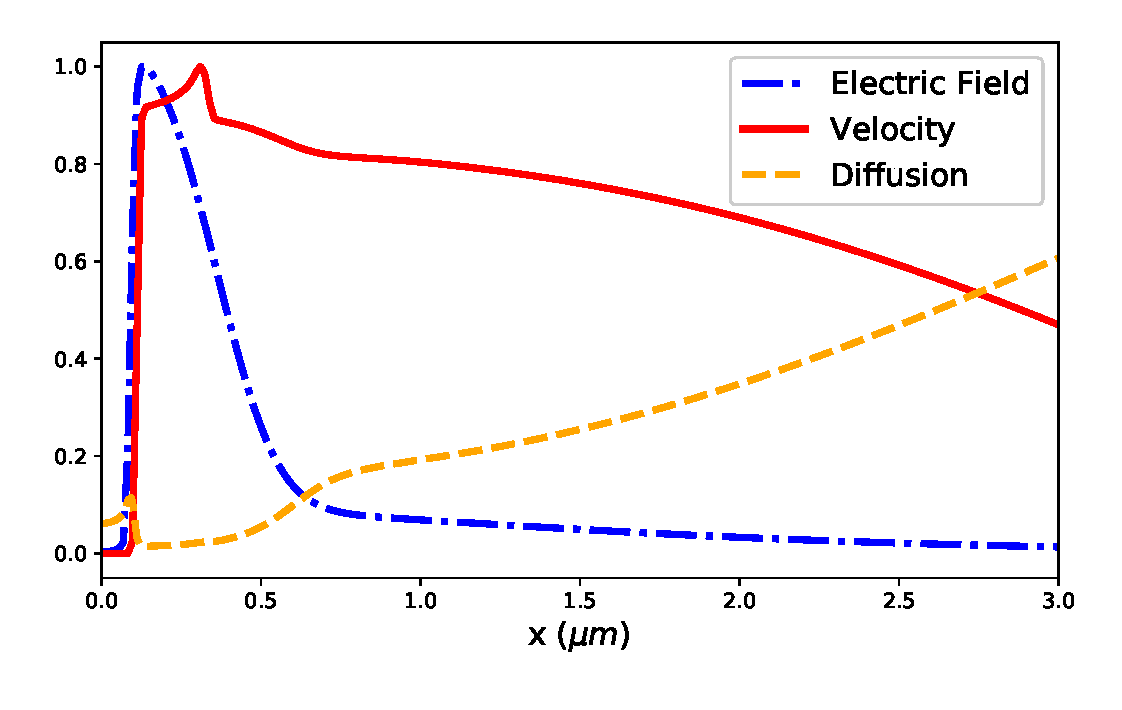
\includegraphics[scale=0.5]{../pictures/NewDiffusionVeloField.eps}
\caption{Normalized Electric Field, Velocity and Diffusion along a streamline}
\label{fig:VelocityDiffusion}
\end{figure}
The equation is solved by the mean of the finite difference method, more precisely we use a modified Crank-Nicholson method that takes into account the variable velocity and diffusion.


%\subsection{Numerical solution}
%First, we discretize the streamline $\Omega$ as \[\Omega_h = \left\lbrace x_s = x_0, x_1, x_2, \cdots, x_{N-1}, x_N = x_{max} \right\rbrace \]
%And time interval as : 
%\[[t_0, t_{max}] = \left\lbrace t_0 = t_0, t_1, t_2, \cdots, t_{M-1}, t_M = t_{max} \right\rbrace \]
%The approximation of the solution is noted :
% \[f(x_i, t_k) \simeq f_i^k \: \: \:   \text{    for } i \in \left\lbrace 0, \cdots, N\right\rbrace  \text{ and } k \in \left\lbrace 0, \cdots, M \right\rbrace  \]
%The equation is solved by the mean of the finite difference method, more precisely we use a modified Crank-Nicholson method. The differentiation of the equation reads : 
%\begin{tiny}
%\useshortskip
%\begin{align*}\label{eq:CrankNicolson}
%\frac{f_i^{k+1} - f_i^{k}}{dt} =& \frac{1}{2} \left[ - u_i \frac{f_{i+1}^{k+1} - f_{i-1}^{k+1}}{2h} 
%				+ D_i \frac{f_{i+1}^{k+1} - 2 f_{i}^{k+1} + f_{i-1}^{k+1}}{h^{2}}  \right] \\
%				+& \frac{1}{2} \left[-f_i^k \frac{u_{i+1} - u_{i-1} }{2h}
%				+ \frac{D_{i+1} - D_{i-1} }{2h} \frac{f_{i+1}^{k+1} - f_{i-1}^{k+1}}{2h} \right] \\ 								
%				+ &\frac{1}{2} \left[ - u_i \frac{f_{i+1}^{k} - f_{i-1}^{k}}{2h} 
%				+ D_i \frac{f_{i+1}^{k} - 2 f_{i}^{k} + f_{i-1}^{k}}{h^{2}} \right] \\
%				+ &\frac{1}{2} \left[-f_i^k \frac{u_{i+1} - u_{i-1} }{2h}
%				+ \frac{D_{i+1} - D_{i-1} }{2h} \frac{f_{i+1}^{k} - f_{i-1}^{k}}{2h} \right] \
%\end{align*}
%\end{tiny}
%It is then straightforward that the resulting scheme will be a linear system to solve with a matrix vector product as right hand side member: 
%\[ A F^{k+1} = B F^k\]


\section{Results and comparisons with experiments}


To validate our models, the simulation results were compared with experimental measurements performed on the wide range of architecture variants described in section \ref{Device}. Where appropriate measurements are repeated on several SPADs to reduce the variability of the results and the values given are the median. 

We first present the PDE results derived from the avalanche breakdown probability simulations described in section \ref{AvaBrP}. A key visualisation of the result is the 2D BrP colour map, which is generated for two different architectures with varying junction size in figure \ref{fig:BrP2DHeatMap}.
\begin{figure}[h!]
\centering
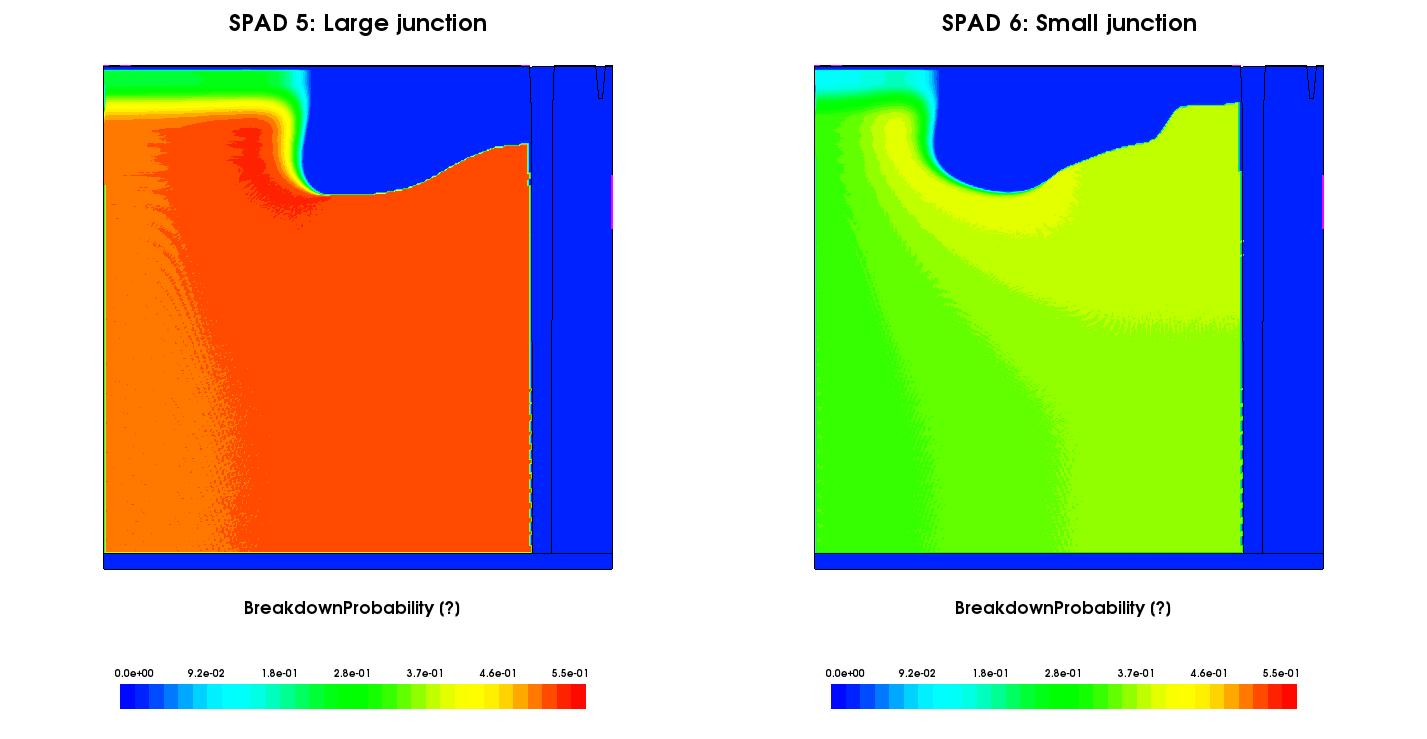
\includegraphics[width=0.9\linewidth]{../pictures/PPVariationNoAxesHorizontalLegend2.jpg}
\caption{2D colour maps of BrP from two design variations with a larger and a smaller avalanche region. BrP is shown at BV+4V and at 333K}
\label{fig:BrP2DHeatMap}
\end{figure}

To verify that the prediction of higher PDE for a smaller junction size is physical, we can extract the integrated PDE for a range of voltages. The resulting curve is shown for the three architectures with junctions of various widths overlaid by the appropriate experimental results in figure \ref{fig:PDEvsVHV}. The PDE values are obtained by multiplying the breakdown avalanche probability by an average optical absorption, found to be 26\% for this architecture.
\begin{figure}[h!]
\centering
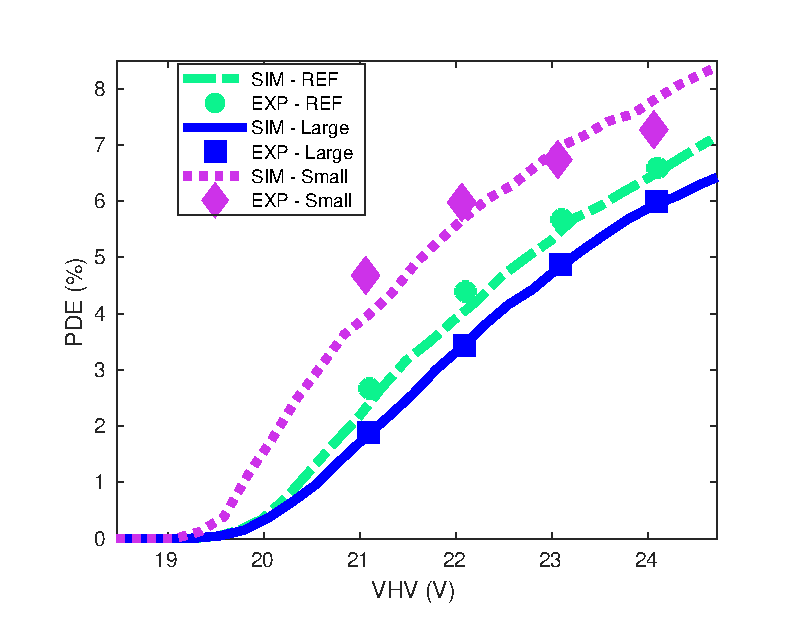
\includegraphics[scale=0.69]{../pictures/000_McIntyre_Bench_GR5_graphs.eps}
\caption{Comparison of PDE measured and simulated on three architecture variations}
\label{fig:PDEvsVHV}
\end{figure}

The comparison was extended to a large set of fifteen different architectures with electric field profiles selected for their wide range of electrostatic characteristics. As shown in figure \ref{fig:PDEcorrel}, which presents the correlation between simulation and experiment at 4V excess voltage, the model was able to predict a significant range of PDE correctly.

\begin{figure}[h]
\centering
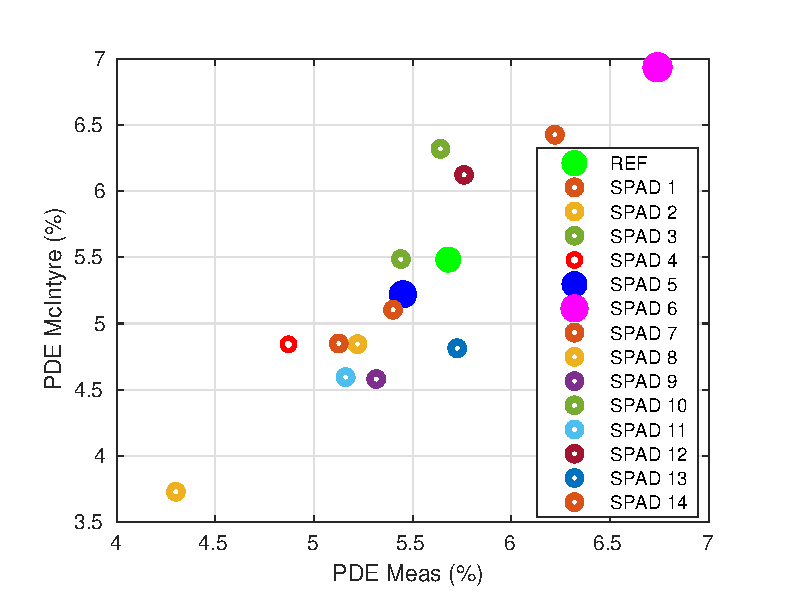
\includegraphics[scale=0.65]{../pictures/000_McIntyre_Bench_GR5_graphs_corel.eps}
\caption{Correlation between simulation and experiment for PDE at BV+4V at 333K for 15 diodes of varying architecture}
\label{fig:PDEcorrel}
\end{figure}

An additional strength of the avalanche breakdown probability methodology is that the breakdown voltage (BV) can be extracted from the PDE vs voltage curve. We define that the device has broken down when a threshold PDE of $1e-5$ is reached, as shown in figure \ref{fig:BVExtract}. The extraction was performed on the same fifteen diodes and the results, shown in figure \ref{fig:BVCorrel}, show the resulting correlation. In particular, the extreme breakdown voltages engineered for SPADs 3 and 4 are predicted by the model with ease. 

\begin{figure}[h!]
\centering
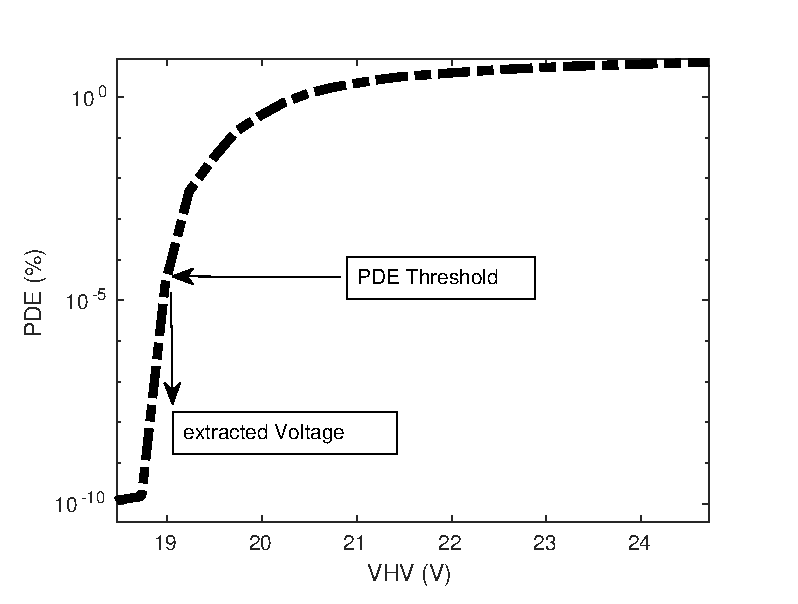
\includegraphics[scale=0.65]{../pictures/000_McIntyre_Bench_Method.eps}
\caption{Method for BV extraction; the threshold defining breakdown is defined at a PDE of $1e-5$}
\label{fig:BVExtract}
\end{figure}

\begin{figure}[h!]
\centering
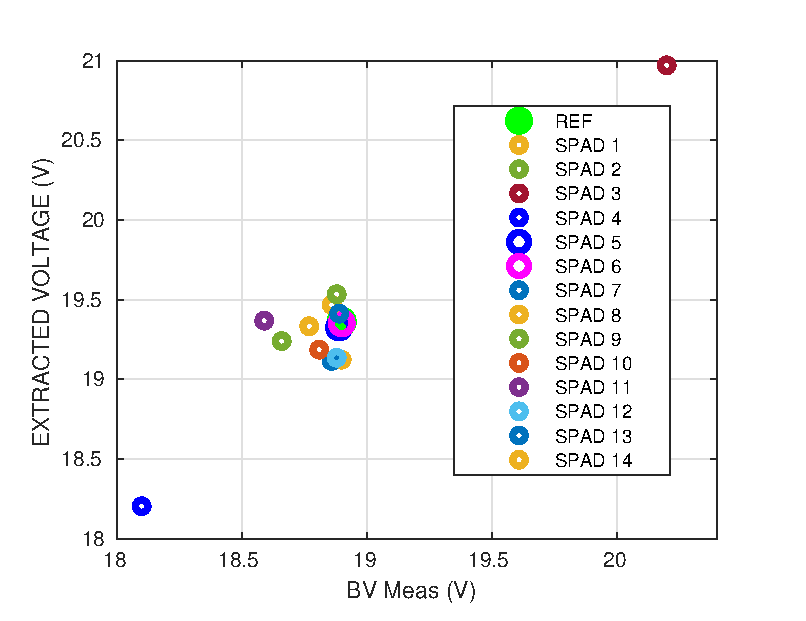
\includegraphics[scale=0.65]{../pictures/000_McIntyre_Bench_GR5_graphs_BV.eps}
\caption{Correlation between simulation and measurements for BV at 333K for 15 diodes of varying architecture}
\label{fig:BVCorrel}
\end{figure}

Finally a comparison between characterisation and simulation was made for the jitter model. Figure \ref{fig:jitter} shows two diodes engineered to exhibit varying jitter profiles. In order to verify that jitter model is valid for a wide range of architectures, the pitch size and a variety of layout parameters were varied. The experimental results for the large diode show a strong initial peak and a rapid decrease in jitter. In contrast, the smaller diode has a much weaker initial peak and a second smaller peak leading to a longer jitter tail. These characteristics are well represented in the simulation results, which shows a second peak for the smaller diode and longer tail. The crossing point between the two curves is also clearly indicated.

\begin{figure}[h!]
\centering
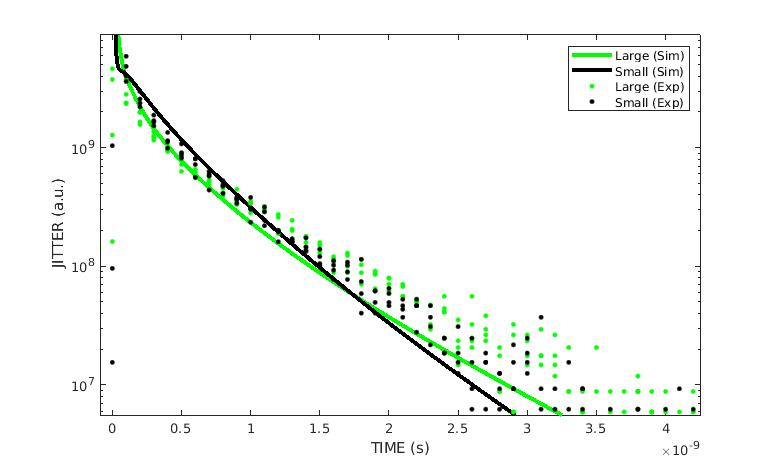
\includegraphics[width=0.9\linewidth]{../pictures/000_JITTER_ESSDERC.jpg}
\caption{Comparison between characterisation and simulation for jitter on a 10um and 5um diode at BV+4V}
\label{fig:jitter}
\end{figure}


The good predictivity shown by both the BrP and jitter models in predicting PDE, BV and jitter characteristics is essential to confirm a clear understanding of the device physics. Furthermore, it allows for many iterations of design optimization without the need for silicon.


\bibliographystyle{ieeetr}
\bibliography{../biblio/essderc2k21}




\end{document}